Neural networks first appeared in literature as early as the 1960's, but until the introduction of NEAT a user had to manually 
estimate the number of nodes needed to solve the problem and how these nodes were connected. In addition the network required
retraining every time new data was presented and failed to properly react to a changing objective function. These issues were
mitigated with the introduction of NEAT in 2002 \cite{stanley2002evolving}. NEAT evolves not only the weights of a network but
the placement of linkages and nodes inside of the network. This process is governed by a memorization genetic algorithm that 
seeks to optimize a user's fitness function. The major advantage of this system is the protection of innovation via speciation.
Speciation allows novel structures to survive long enough to eventually find a more optimal solution to the user's problem. 
This is important to the facial deformation problem as novel facial structures would be lost in any algorithm that erratically
explores the search space. Introducing the concept of speciation along with fitness sharing smooths out the exploration of the
search space and allows semi-guided search to take place. The biggest issue with NEAT is that it still requires some
user input in the form of an objective. This domain input is needed in order for NEAT to decide if one structure is more
viable than another, but a function comparing the novelty of images is currently not known. 

\begin{figure}
 \centering
 \label{fig:paper:CPPN}
 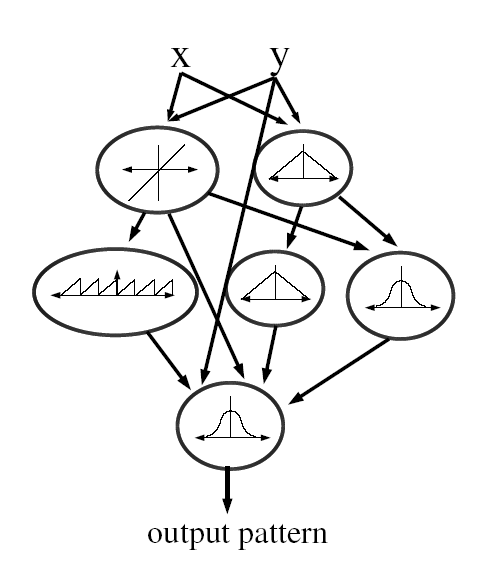
\includegraphics[width=0.4\textwidth]{../../rec/paper/cppn.png}
 \caption{A graph abstraction of a compositional pattern producing network. The CPPN abstraction can be applied to a neural network type structure as the graph depicts \cite{stanley2002evolving}}
\end{figure}

Due to the limitations of the NEAT process a second abstraction must be introduced in order to properly explore the facial 
deformation problem. CPPNs are indirectly encoded developmental networks that describe in an indirect manner the representation
of a more complicated entity \cite{stanley2007compositional}. CPPNs eliminate two limitations: the first
being the requirement of a homogeneous activation function in nodes; the second is sampling among a continuum rather than
discrete points. Because CPPNs describe how a function evolves rather than how to evaluate a function CPPNs represent a
different structure then that of artificial neural networks but one that can utilize the same structure of the networks
\ref{fig:paper:CPPN}. The combination of NEAT with the CPPN abstraction allows for greater ability to come up with a
generational model for how a function develops \cite{stanley2007compositional}. This process also allows for simplification
of the fitness sharing metric involved in speciation of the neural networks. In lieu of a domain restricted optimization
function the distance between the two networks can be used to properly speciate the evolved networks \cite{stanley2007compositional}.
Another advantage of the algorithm is due to the domain of images: as images change in resolution and density more
input neurons are not required as would be under traditional neural network architectures. The CPPN ignores the resolution
of the image and can generalize how the image is produced thus saving valuable computational time. In addition, the process of
including symmetrical activation functions with a generative process allows exclusion of large amounts of the search space
allowing more efficient search for interesting artifacts. To this end the CPPN/NEAT architecture allows interesting facial
deformations to be discovered by the user in a timely and rigorous manner.

\begin{figure*}
 \centering
 \label{fig:paper:picbreed}
 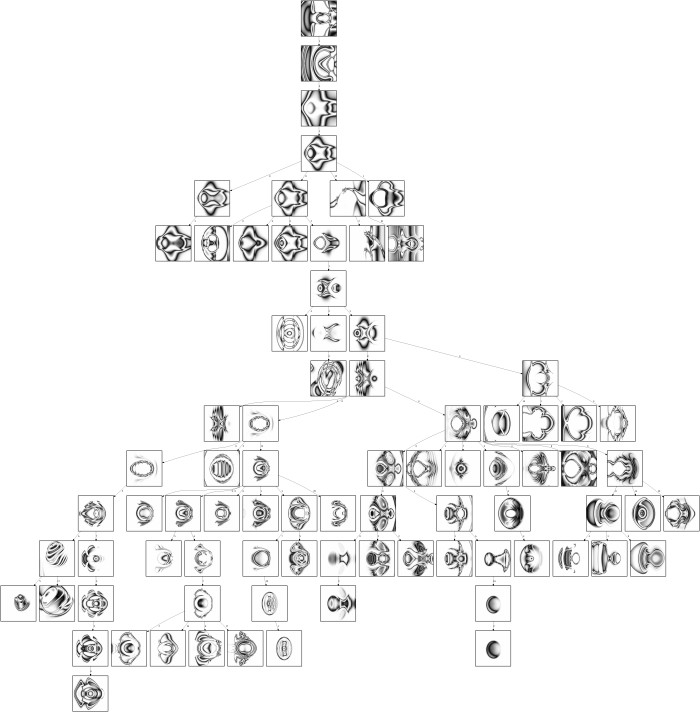
\includegraphics[width=0.7\textwidth]{../../rec/paper/picbreed.jpg}
 \caption{From PicBreeder: A graph abstraction of a compositional pattern producing neural network. The CPPN abstraction can be applied to a neural network type structure as the graph depicts \cite{stnaleypicbreed}}
\end{figure*}

There still exists a issue to implementation of the algorithm and that is the objective function. The novelty of the deformed human face is 
difficult to express in mathematical terms. Due to this limitation evolving interesting deformations with CPPN/NEAT is impossible.
There exists another abstraction that of Interactive Evolutionary Computation or IEC, IEC supplements a mathematical objective function
for one driven by a human operator.Instead of performing a straight optimization route on images, Humans perform a meta-heuristic like search of the novel
spaces which encodes the optimal function this performs a search for interesting or novel entries \cite{lehman2010efficiently} \cite{li2009innovative}.  The CPPN/NEAT architecture has already been applied successfully to this domain with the inclusion of IEC \cite{secretan2008picbreeder}. PicBreeder allows for anyone with an internet connection to evolve images from simple functions into genetic art. The users of the site effectively
perform a modified Gibbs sampling algorithm on the search space of interesting images. This gives the PicBreeder program insight
into the higher dimensional fitness function will still allowing CPPN/NEAT to evolve the underlying image representation. PicBreeder
becomes a lesson in how to efficiently search through possible images, and its process becomes a cornerstone of the facial
deformation discovery process.